\chapter{Badania}

\section{Przeprowadzone badania}

Zgodnie z założeniami, badania przeprowadzono dla 5 różnych liczb neuronów w warstwie ukrytej: \textbf{5, 10, 20, 40, 60}.

Badania rozpoczynają się od iteracji przez wybrane liczby neuronów w warstwie ukrytej. W każdej iteracji uruchamiane są testy dla różnych liczb cech, począwszy od 1 a skończywszy na maksymalnej liczbie cech w zbiorze testowym, w tym wypadku 32. W tym momencie następuje n-krotne wykonanie uczenia i klasyfikacji, a z n-próbek wyciągane są wartości skrajne min-max, liczona jest średnia oraz odchylenie standardowe. Uzyskane w ten sposób wartości służą w późniejszym etapie do odpowiedniego zobrazowania wyników na wykresach. Na potrzeby badań uznano, że 5 powtórzeń będzie wystarczające.

Oba algorytmy uruchamiano z różnymi wartościami stałych parametrów. Oto lista niezmiennych parametrów z jakimi uruchamiano algorytm \texttt{BP}:

\begin{table}[h!]
    \centering
    \caption{Parametry algorytmu \texttt{BP}.}
    \begin{tabular}{p{3cm}p{2cm}p{11cm}}
        \toprule
        \textbf{Parametr} & \textbf{Wartość} & \textbf{Opis} \\
        \midrule
        \texttt{algorithm} & \texttt{sgd} & Algorytm działania (\textit{stochastic gradient descent}). \\
        \texttt{max\_iter} & \texttt{10000} & Maksymalna liczba iteracji. \\
        \texttt{alpha} & \texttt{1e-6} & Parametr regularyzacji L2. \\
        \texttt{learning\_rate} & \texttt{constant} & Tempo uczenia. \\
        \texttt{activation} & \texttt{logistic} & Funkcja aktywacji warstwy ukrytej. \\
        \texttt{random\_state} & \texttt{None} & Ziarno dla generatora liczb losowych. \\
        \bottomrule
    \end{tabular}
\end{table}

Dla algorytmu \texttt{ELM} powyższe parametry były takie same, bądź nie trzeba było ich wprowadzać, z jedną różnicą, gdzie jako funkcji aktywacji użyto funkcję \texttt{multiquadric}.

\newpage

\section{Porównanie algorytmów}

Dla 5 neuronów w warstwie ukrytej zauważyć można, że oba algorytmy osgiągneły prawie takie same wyniki oscylujące w okolicy 76\%, niezależne od liczby wyselekcjonowanych cech.

Również czasy uczenia okazały się bardzo podobne. Wystąpiły tutaj jednakże większe fluktuacje, spowodowane przede wszystkim niedokładnością w mierzeniu bardzo małych czasów (rzędu 0.5 milisekundy) oraz dużym odchyleniem standardowym sygnalizowanym na wykresie przez słupki błędu.

Największą różnicę zauważyć jednak można w czasach uczenia się, gdzie algorytm \texttt{ELM} osiągnął o wiele lepsze czasy rzędu 2 milisekund od algorytmu \texttt{BP}, którego średni czas oscylował w okolicy 130 milisekund. Zauważyć zatem można wyraźnie, że algorytm \texttt{ELM} jest średnio 65 razy szybszy od algorytmu \texttt{BP}.

\begin{figure}[h!]
	\centering
	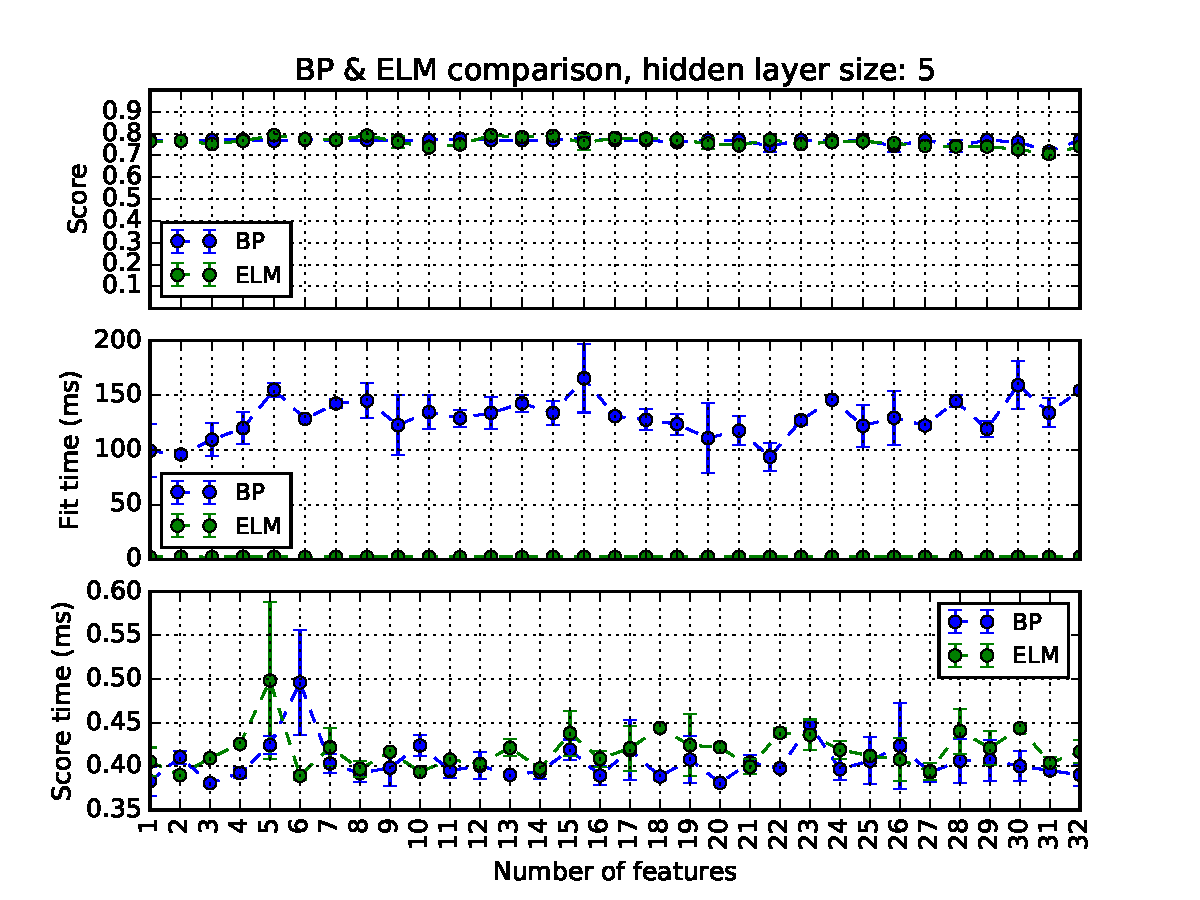
\includegraphics[width=1.0\linewidth]{img/bp_elm_5.pdf}
	\label{Rysunek}
	\caption{5 neuronów w warstwie ukrytej - porównanie obu algorytmów}
\end{figure}

\newpage

Dla 10 neuronów w warstwie ukrytej zachodzą te same zależności. Widoczny jest jednak nieznaczny wzrost czasu uczenia dla algorytmu \texttt{BP} do około 250 milisekund w okolicy 10-14 wyselekcjonowanych cech. Algorytm \texttt{ELM} pozostaje bez zmian.

\begin{figure}[h!]
	\centering
	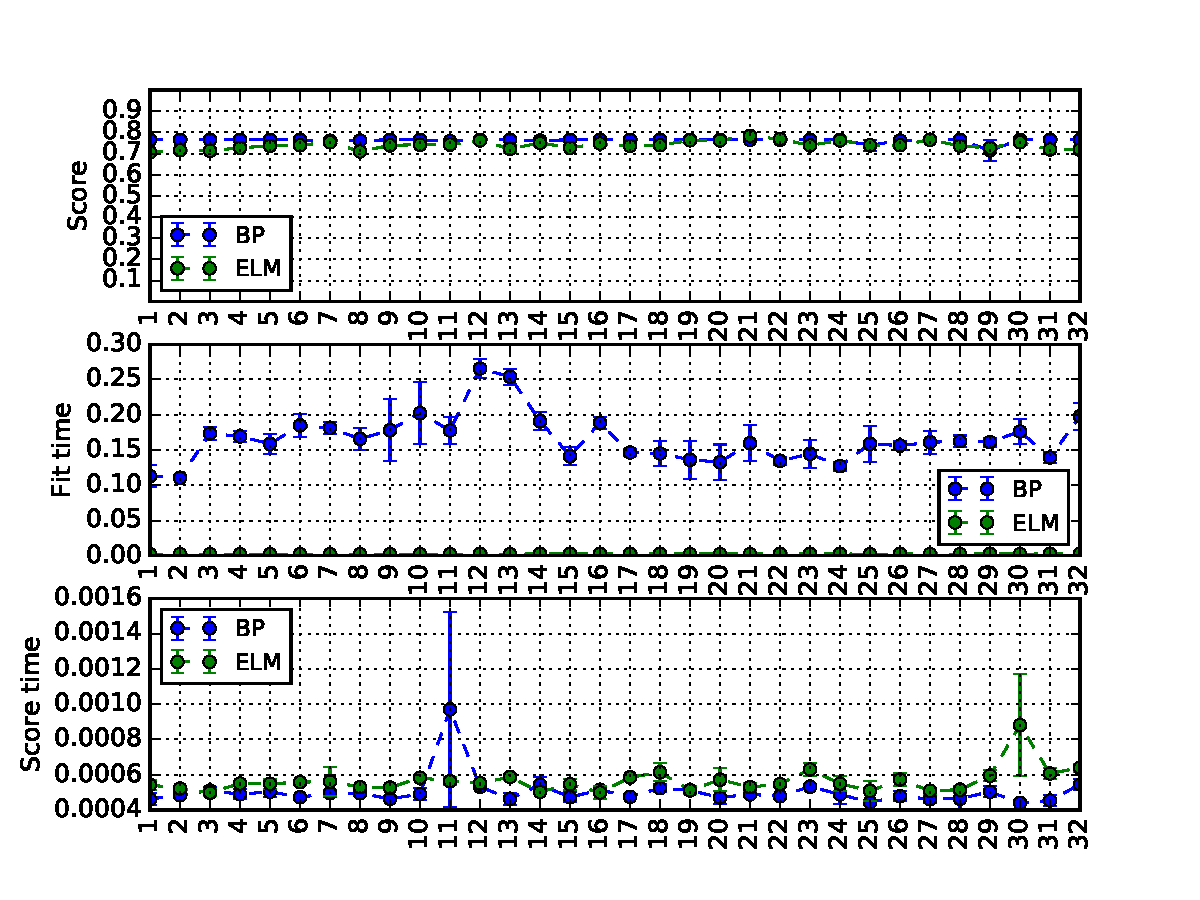
\includegraphics[width=1.0\linewidth]{img/bp_elm_10.pdf}
	\label{Rysunek}
	\caption{10 neuronów w warstwie ukrytej - porównanie obu algorytmów}
\end{figure}

\newpage

Dla 20 neuronów w warstwie ukrytej zdecydowanie zauważyć już można tendencję w czasie uczenia algorytmu \texttt{BP}, gdzie do około 7 wyselekcjonowanych cech czas znacząco wzrasta, później do około 16 sech pozostaje względnie stały, następnie maleje i od 22 cech utrzymuje się już na sałym, niskim poziomie rzędu 100 milisekund. Wytłumaczyć tę zależność można zjawiskiem przeuczenia, gdzie algorytm osiągnął lokalne minima, a następnie je wykorzystywał przy kolejnych uczeniach.

\begin{figure}[h!]
	\centering
	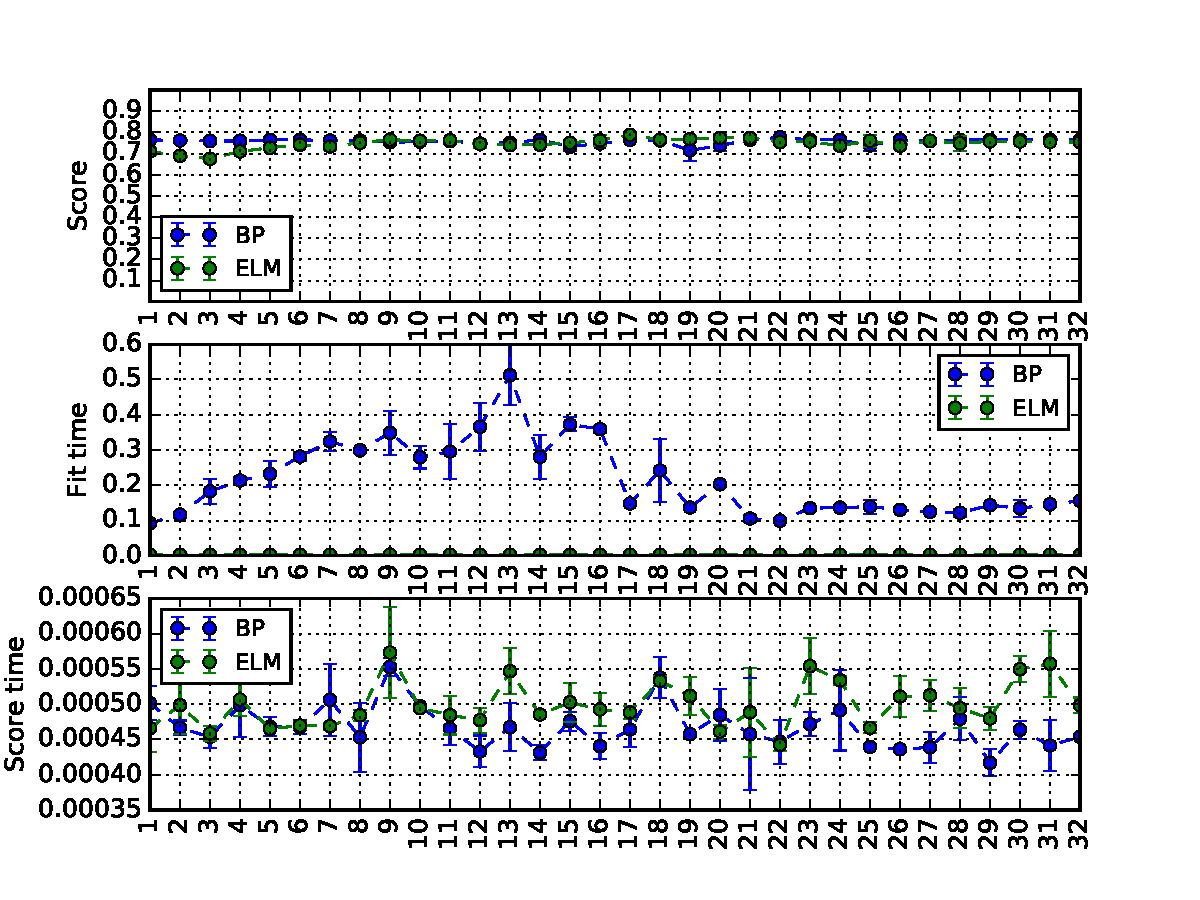
\includegraphics[width=1.0\linewidth]{img/bp_elm_20.pdf}
	\label{Rysunek}
	\caption{20 neuronów w warstwie ukrytej - porównanie obu algorytmów}
\end{figure}

\newpage

Dla 40 neuronów w warstwie ukrytej widać już bardzo wyraźnie zauważone wcześniej tendencje dla algorytmu \texttt{BP}. Reszta zależności pozostaje bez zmian.

\begin{figure}[h!]
	\centering
	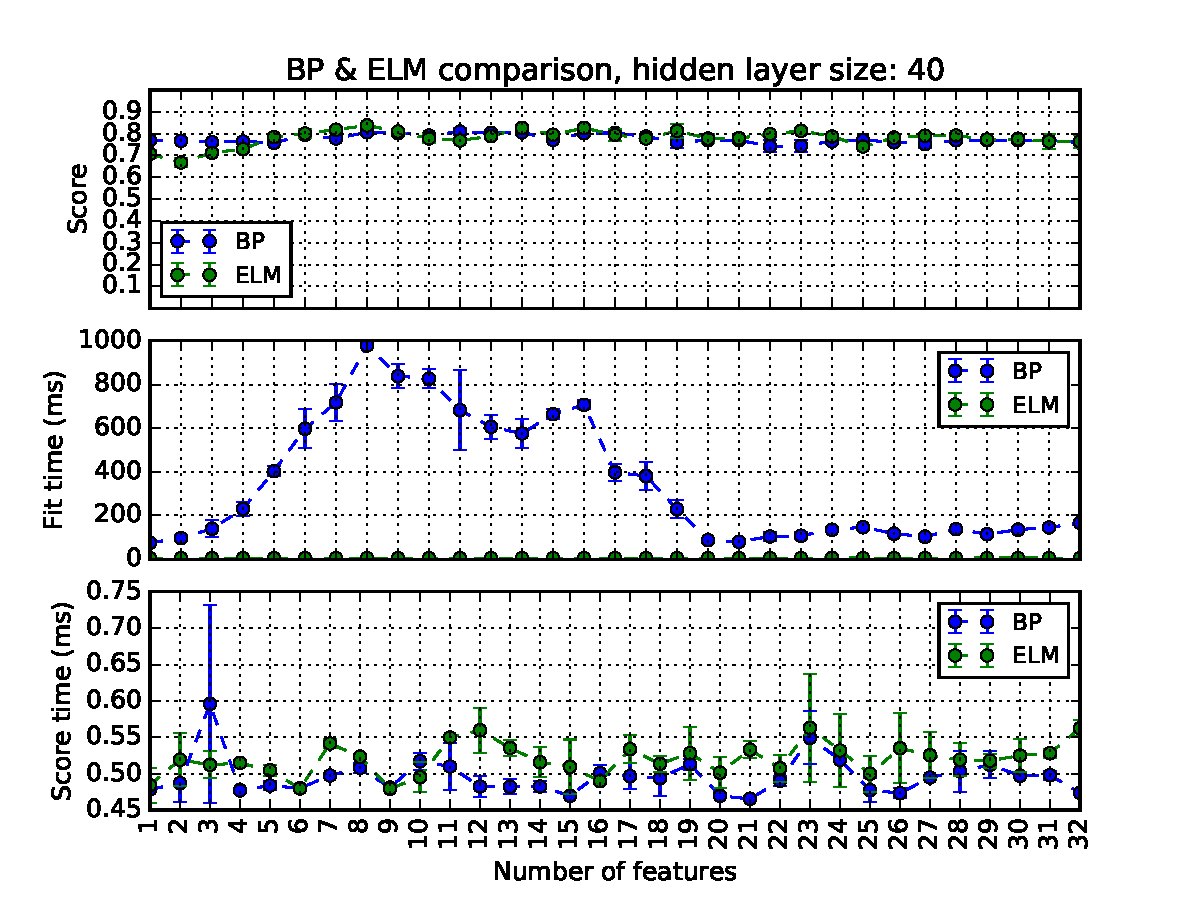
\includegraphics[width=1.0\linewidth]{img/bp_elm_40.pdf}
	\label{Rysunek}
	\caption{40 neuronów w warstwie ukrytej - porównanie obu algorytmów}
\end{figure}

\newpage

Dla 60 neuronów w warstwie ukrytej widać, że powyższe zależności pogłębiły się znacząco i czas uczenia algorytmu \texttt{BP} osiągał 1.2 sekundy. 

\begin{figure}[h!]
	\centering
	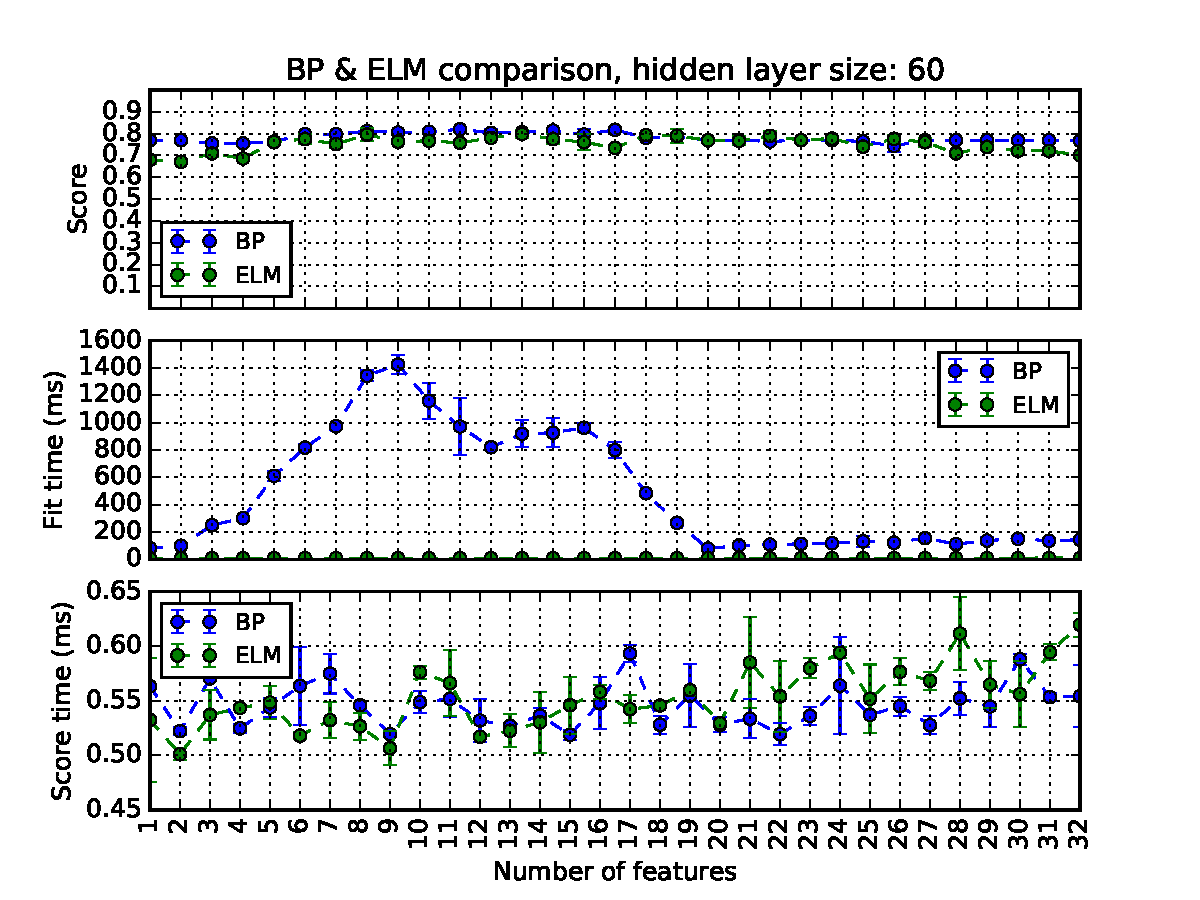
\includegraphics[width=1.0\linewidth]{img/bp_elm_60.pdf}
	\label{Rysunek}
	\caption{60 neuronów w warstwie ukrytej - porównanie obu algorytmów}
\end{figure}

\newpage

\section{Selekcja cech}
Selekcja cech polega na wybieraniu podzbioru cech w celu ograniczenia czasu uczenia, uproszczenia modelu oraz minimalizacji zjawiska przeuczenia.

W projekcie skorzystano z klasy \texttt{SelectKBest}, z modułu \texttt{sklearn.feature\_selection}.
\begin{figure}[h!]
	\centering
	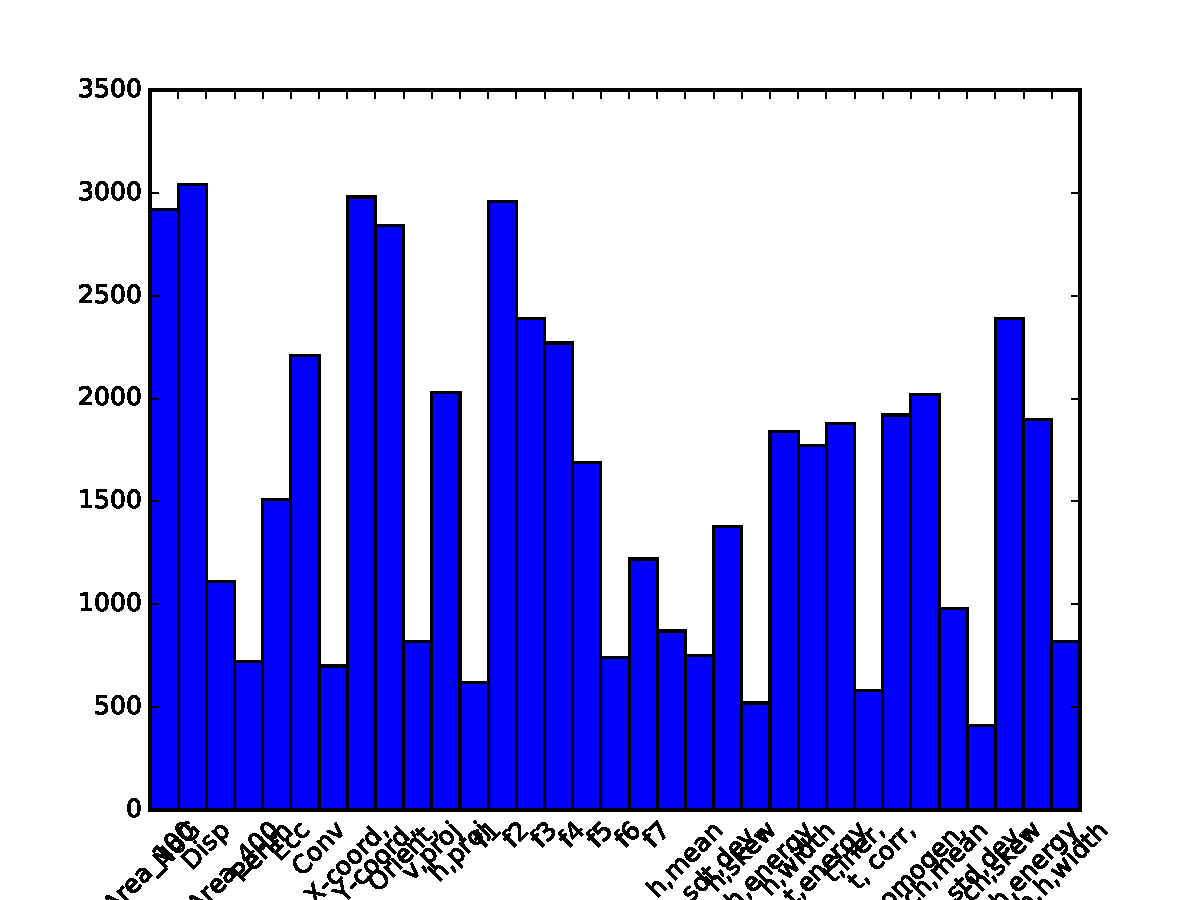
\includegraphics[width=1.0\linewidth]{img/features.pdf}
	\label{Rysunek}
	\caption{Częstość wybierania cech}
\end{figure}

\newpage

\section{Macierz pomyłek}
Macierz pomyłek umożliwia zobrazowanie jak dobrze klasyfikator radzi sobie ze swoim zadaniem.

Dla problemu z dwiema klasami -- tak jak w aktualnie rozpatrywanym problemie -- macierz dzieli się na cztery części, w których zliczane są obiekty sklasyfikowane poprawnie -- umieszczone na przekątnej macierzy -- oraz błędnie -- umieszczone poza przekątną.

W projekcie skorzystano z funkcji \texttt{confusion\_matrix}, z modułu \texttt{sklearn.metrics}.
\begin{figure}[h!]
	\centering
	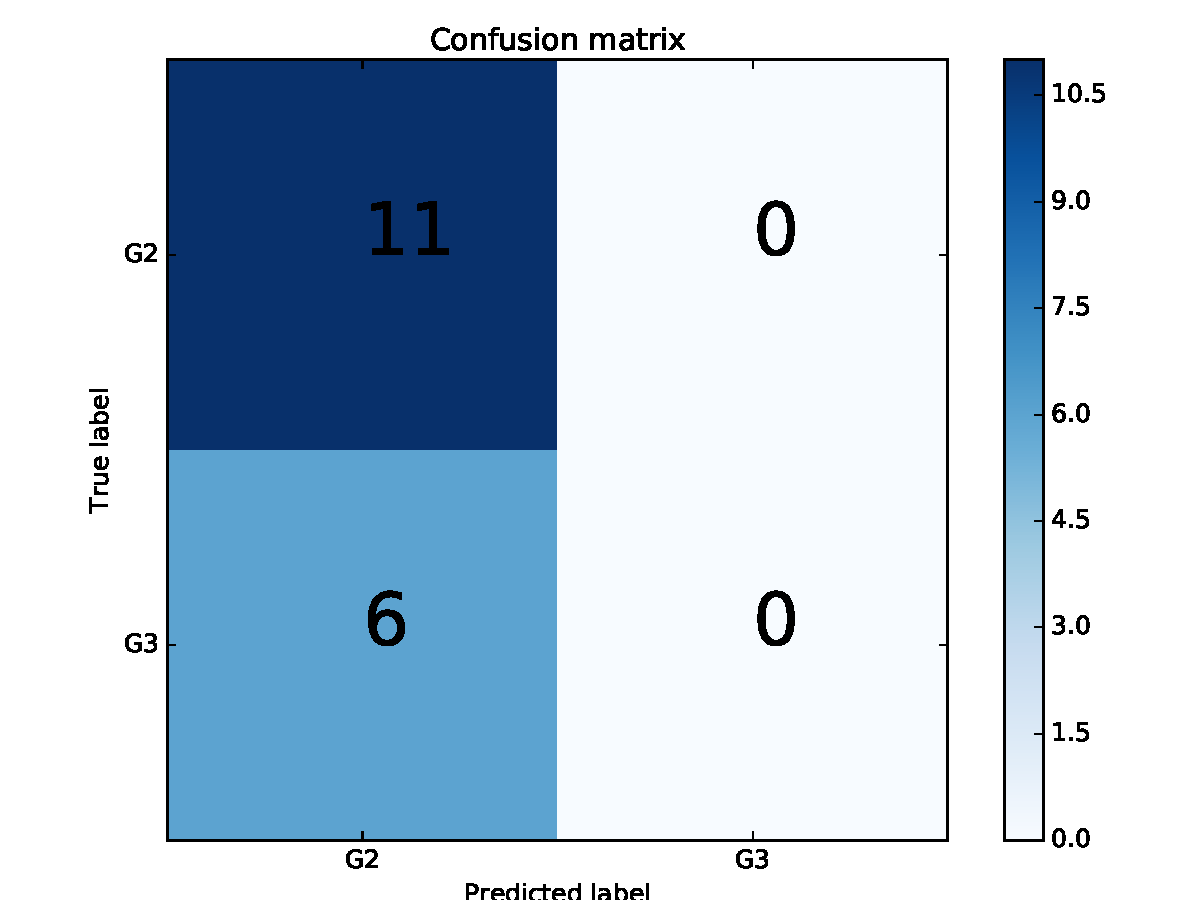
\includegraphics[width=1.0\linewidth]{img/conf_matrix.pdf}
	\label{Rysunek}
	\caption{Przykładowa macierz pomyłek}
\end{figure}